\documentclass[a4paper,14pt]{extreport} % формат документа

\usepackage{amsmath}
\usepackage{cmap} % поиск в ПДФ
\usepackage[T2A]{fontenc} % кодировка
\usepackage[utf8]{inputenc} % кодировка исходного текста
\usepackage[english,russian]{babel} % локализация и переносы
\usepackage[left = 2cm, right = 1cm, top = 2cm, bottom = 2 cm]{geometry} % поля
\usepackage{listings}
\usepackage{graphicx} % для вставки рисунков
\usepackage{amsmath}
\usepackage{float}
\usepackage{multirow}
\graphicspath{{pictures/}}
\DeclareGraphicsExtensions{.pdf,.png,.jpg}
\newcommand{\anonsection}[1]{\section*{#1}\addcontentsline{toc}{section}{#1}}

\lstset{ %
	language=Prolog,                % Язык программирования 
	numbers=left,                   % С какой стороны нумеровать          
	frame=single,                    % Добавить рамку
}

\begin{document}
\begin{titlepage}

    \begin{table}[H]
        \centering
        \footnotesize
        \begin{tabular}{cc}
            \multirow{8}{*}{
\includegraphics[scale=0.35]{bmstu.jpg}}
            & \\
            & \\
            & \textbf{Министерство науки и высшего образования Российской Федерации} \\
            & \textbf{Федеральное государственное бюджетное образовательное учреждение} \\
            & \textbf{высшего образования} \\
            & \textbf{<<Московский государственный технический} \\
            & \textbf{университет имени Н.Э. Баумана>>} \\
            & \textbf{(МГТУ им. Н.Э. Баумана)} \\
        \end{tabular}
    \end{table}

    \vspace{-2.5cm}

    \begin{flushleft}
        \rule[-1cm]{\textwidth}{3pt}
        \rule{\textwidth}{1pt}
    \end{flushleft}

    \begin{flushleft}
        \small
        ФАКУЛЬТЕТ
        \underline{<<Информатика и системы управления>>\ \ \ \ \ \ \ 
        \ \ \ \ \ \ \ \ \ \ \ \ \ \ \ \ \ \ \ \ \ \ \ \ \ \ \ \ \ \ \ 
    \ \ \ \ \ \ \ \ \ \ \ \ \ \ \ } \\
        КАФЕДРА
        \underline{<<Программное обеспечение ЭВМ и
        информационные технологии>>
        \ \ \ \ \ \ \ \ \ \ \ \ \ \ \ \ \ \ \ \ }
    \end{flushleft}

    \vspace{4cm}

    \begin{center}
        \textbf{Лабораторная работа № 12} \\ 
        \hfill
        
        \textbf{Структура программы на Prolog} \\
        \vspace{0.5cm}
        \textbf{} \\
    \end{center}

    \vspace{4cm}

    \begin{flushleft}
        \begin{tabular}{ll}
            \textbf{Дисциплина} & Функциональное и логическое программирование \\
            \textbf{Студент} & Сиденко А.Г. \\
            \textbf{Группа} & ИУ7-63Б \\
            \textbf{Преподаватель} & Толпинская Н.Б., Строганов Ю.В.  \\
        \end{tabular}
    \end{flushleft}

    \vspace{4cm}

   \begin{center}
        Москва, 2020 г.
    \end{center}

\end{titlepage}

\textbf{Задание}

Составить программу – базу знаний, с помощью которой можно определить, например, множество студентов, обучающихся в одном ВУЗе. Студент может одновременно обучаться в нескольких ВУЗах. Привести примеры возможных вариантов вопросов и варианты ответов (не менее 3-х). Описать порядок формирования вариантов ответа.

\textbf{Программа <<База данных ВУЗов>>}

\begin{lstlisting}
domains
  name, university = string.
predicates
  universe(name, university).
clauses
  universe("Ellen", "BMSTU").
  universe("Ellen", "MSU").
  universe("John", "MSU").
  universe("Tom", "MFTI").
  universe("Tom", University) :- universe ("John", University).
  universe("Eric", "HSE").
  universe("Eric", "BMSTU").
  universe("Mark", "MIFI"). 
  universe("Mark", "HSE"). 
  universe("Mark", University) :- universe ("Tom", University).
  universe("Bill", University) :- universe ("Tom", University). 
\end{lstlisting}

\textbf{Примеры работы}

\begin{enumerate}
\item Определение в каких университетах учится Mark. 

Цель системы состоит в том, чтобы на поставленный вопрос найти возможность, исходя из базы знаний, ответить <<Да>>. В нашем случае система настроена в режим получения всех возможных вариантов ответа <<Да>> на поставленный вопрос.

\begin{lstlisting}
goal
  Name = "Mark",
  write(Name, " universities: "), nl,
  universe(Name, University).
\end{lstlisting}


\includegraphics{ex1}

\item Определение кто учится в BMSTU. 

\begin{lstlisting}
goal
  University = "BMSTU",
  write(University, " students: "), nl,
  universe(Name, University).
\end{lstlisting}

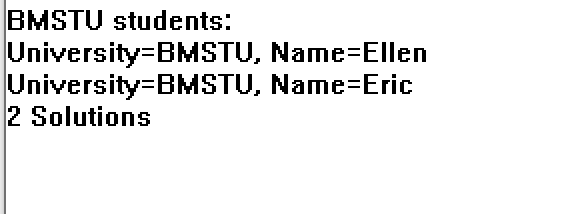
\includegraphics{ex2}

\item Определение учится ли Bill в BMSTU. 

В данном варианте раздела GOAL система не найдет возможность ответить <<Да>>. В результате полученный ответ. 

\begin{lstlisting}
goal
  Name = "Bill",
  University = "MSTU",
  write(Name, " is student ", University, "?"), nl,
  universe(Name, University).
\end{lstlisting}


\includegraphics{ex3}

\end{enumerate}

\textbf{Ответы на вопросы}

что собой представляет программа на Prolog, какова ее структура. Как она реализуется, как формируются результаты работы программы. 

\textbf{Программа на Prolog представляет собой:} базу знаний и вопрос. База знаний содержит истинностные знания, используя которые программа выдает ответ на запрос. 

Основным элементом языка является терм. Терм – это: константа, переменная, составной терм. С помощью термов и более сложных конструкций языка Prolog – фактов и правил <<описываются>> знания о предметной области, т.е. база знаний. Используя базу знаний, система Prolog будет делать логические выводы, отвечая на наши вопросы. 

Программа на Prolog состоит из разделов. Каждый раздел начинается со своего заголовка. 

\textbf{Структура программы }
\begin{enumerate}
\item директивы компилятора -- зарезервированные символьные константы
\item CONSTANTS -- раздел описания констант
\item DOMAINS -- раздел описания доменов
\item DATABASE -- раздел описания предикатов внутренней базы данных
\item PREDICATES -- раздел описания предикатов
\item CLAUSES -- раздел описания предложений базы знаний
\item GOAL -- раздел описания внутренней цели (вопроса).
\end{enumerate}

В программе не обязательно должны быть все разделы.

С помощью подбора ответов на запросы он (Prolog, программа) извлекает хранящуюся (известную в программе) информацию. Одной из особенностей Prolog является то, что при поиске ответов на вопрос, он рассматривает альтернативные варианты и находит все возможные решения (методом проб и ошибок) -- множества значений переменных, при которых на поставленный вопрос можно ответить -- <<да>>.

Поиск содержательного ответа на поставленный вопрос, с помощью имеющейся базы знаний, фактически заключается в поиске нужного знания, но какое знание понадобится – заранее неизвестно. Этот поиск осуществляется формально с помощью механизма унификации. Упрощенно, процесс унификации можно представить как формальный процесс сравнивания терма вопроса с очередным термом знания. При этом, знания по умолчанию просматриваются сверху вниз. В процессе сравнивания для переменных «подбираются», исходя из базы знаний, значения или подтверждается истинность вопроса. 

\textbf{Переменные}

При поступлении вопроса с переменной в Пролог-систему. Например:
\begin{lstlisting}
  universe("Mark", X).
\end{lstlisting}

X -- переменная, входящая в вопрос, изначально является неконкретизированной. Пролог просматривает базу данных в поисках факта, сопоставимого с вопросом. Если неконкретизированная переменная появляется в качестве одного из аргументов, то Пролог считает, что такой аргумент сопоставим с любым другим аргументом, находящимся в том же факте. При обнаружении такого факта переменная X становится конкретизированной, обозначая объект, являющийся вторым аргументом найденного факта и устанавливает в этом месте маркер.

Так как, в нашем случае мы ищем все возможные варианты, именно с места отмеченного маркером Пролог начнет поиск. 
\end{document}